\section{Additional Theoretical Analysis and Proofs}
\label{sec:appendix-theory}

\subsection{Rationale for Rational-valued Model Functions}
\label{sec:real-valued-distributions}

Defining Kolmogorov complexity for a function $f: \gX \rightarrow \R$ with a countable domain but real-valued range is slightly more complicated than for functions with countable (e.g. rational-valued) outputs, but we can accomplish this by considering the shortest program $z$ for a given universal prefix Turing machine $T$ that can approximate $f$ to an arbitrary degree of precision $a \in N$ specified as an additional input:
\begin{equation}
    K(f) = \min \{|z| : \forall x \in \gX,a \in \N~~ \left| T(e_{(\gX \times \N)}(x,a),z) - f(x) \right| \leq 1 / a \}.
\label{eq:kolmogorov-real-valued-function}
\end{equation}

Given this definition, we could define two-part and variational codes with respect to model functions with real-valued logits, analogously to those defined with respect to model functions with rational-valued logits. However, this leads to significantly greater theoretical complexity with limited practical benefit, given that real-world neural networks represent logits with finite precision, and any real-valued function can be approximated to an arbitrary degree of precision by a rational-valued function.

\subsection{Note on ``Universal'' Terminology}
\label{sec:universal-terminology}

The term \emph{universal} is overloaded in the context of codes and compression schemes, with different usages varying with respect to the scope (the class of codes/models being compared against) and the nature of the performance guarantee. Our usage of the term in this paper follows the use of the term in the algorithmic information theory literature to describe the \emph{universality} of Kolmogorov complexity with respect to any computable prefix code, up to an additive constant. We extend this notion to slightly restricted sets of prefix codes, i.e. the specific classes of two-part, Bayesian, and variational codes discussed in this paper.

In contrast, the term \emph{universal code} also appears in the MDL literature~\citep{grunwald2004tutorial} to describe codes that are universal with respect to a specific set of candidate codes, in the sense of offering as much compression as any candidate code, up to a factor that is typically logarithmic with respect to the size of the candidate set or data sample. The term ``universal code'' is also used to describe prefix codes for integers, such as Elias codes, which offer asymptotic guarantees relative to any other prefix code assuming a monotonically decreasing probability distribution over the integers. 

\subsection{Model Functions and Notation}
\label{sec:reference-machine-and-notation}

Here we introduce standard encodings, $e_\gX$ and $e_\gL$, used to define the Kolmogorov complexity of model functions, $\gF : \gX \rightarrow \gL$, introduced in Section~\ref{sec:problem-setting}. Let us denote the class of universal prefix Turing machines compatible with these encodings as $\gT$, with the specific assumptions specified in the following paragraphs. Recall that the specific choice of universal prefix Turing machine, and encoding functions $e_\gX$ and $e_\gL$, only affect the resulting definition of Kolmogorov complexity by an additive term (\ref{sec:background-kolmogorov-complexity}), which does not affect the main inequalities we are interested in proving, which hold up to an additive term. Therefore we choose encodings to simplify the construction of a function $\zmap$ introduced later (\ref{sec:zmap-details}), which generates Transformer parameters to emulate a prefix Turing machine.

\paragraph{Input encoding} Let $\gV$ be a vocabulary of input tokens. We assume some one-to-one encoding of inputs $e_\gX : \gX \rightarrow \gV^*$ as a token sequence, which is represented on the input tape. For generality, we do not necessarily assume the input vocabulary is binary, and assume the input tape of any $T \in \gT$ has a number of symbols greater than or equal to $|\gV|$.

\paragraph{Output encoding} Recall that the output of a model function is a tuple of rational-valued logits, with one logit for each element in the output space $\gY$, i.e. $\gL = \mathbb{Q}^{|\gY|}$. We assume that any $T \in \gT$ has $|\gY|$ write-once, unidirectional output tapes, with each logit $\in \mathbb{Q}$ encoded on a separate output tape in the following format. Let $s \in \{ 0,1 \}$ denote the sign of the logit, $\texttt{numerator} \in \N_0$ be the numerator and $\texttt{denominator} \in \N$ be the denominator. The logit is then encoded on the output tape as:
\begin{equation}
s, \overbrace{1, 1, \cdots, 1}^{\texttt{numerator}}, 0, \overbrace{1, 1, \cdots, 1}^{\texttt{denominator}-1},
\end{equation}
followed by blank symbols.
Therefore, $e_\gL : \mathbb{Q}^{|\gY|} \rightarrow (\B)^{|\gY|}$.

\paragraph{Shorthand notation} We introduce the following shorthand notation related to prefix Turing machines and the encoding functions introduced above.

First, let us define a model function $f_T^z \in \gF$ computed by $T \in \gT$ with program $z$ as follows:
\begin{equation}
    f_T^z(x) = e_\gL^{-1}\left( T(e_{\gX}(x),z) \right).
\end{equation}

Next, let us define the set of programs where $T \in \gT$ halts with a valid output for any input:
\begin{equation}
    \gZ_T = \{ z : \forall x \in \gX,~T(e_\gX(x), z) \in \dom(e_\gL) \}.
\end{equation}

Additionally, let us denote the set of programs where $T \in \gT$ halts with a valid output for any input \emph{under resource bound $R$} as:
\begin{equation}
    \gZ_{T,R} = \{ z : \forall x \in \gX,~T_R(e_\gX(x), z) \in \dom(e_\gL) \}.
\end{equation}

Note that we can rewrite the definitions of Kolmogorov complexity with respect to these definitions.
\begin{equation}
    K_T(f) = \min_{z \in \gZ_T  ~:~ f_T^z = f} |z|,
\end{equation}
or $\infty$ if no such $z$ exists, and similarly: 
\begin{equation}
    K_{T,R}(f) = \min_{z \in \gZ_{T,R}  ~:~ f_T^z = f} |z|,
\end{equation}
or $\infty$ if no such $z$ exists, where $f_T^z = f$ denotes that $\forall x \in \gX,~f_T^z(x) = f(x)$.

\subsection{Analysis of Two-Part Codes}

Here we provide the proof of Proposition~\ref{thm:universal-two-part-existence}, along with supporting lemmas and related analysis of two-part codes.

\subsubsection{Lemmas~\ref{lemma-two-part-f} and ~\ref{lemma-two-part-f2}}

We introduce the following lemmas to support our later proofs.

\begin{defn}[description length of a model function]
The \emph{description length of a model function} $f$ under code $M$, denoted $L^\gF_M(f)$, is the codelength of the shortest hypothesis that maps to $f$:
\begin{equation}
    L^\gF_{M}(f) := \min_{h \in \gH_{M}  ~:~ m_M(h)=f} -\log_2 \alpha_M(h).
    \label{eq:function-description-length}
\end{equation}
\end{defn}

\begin{lemma}
\label{lemma-two-part-f}
The minimum codelength of a two-part code $M$ can be expressed as a minimization over the set of model functions realized by $M$:
\begin{equation}
    L_{M}^{\bigast,\text{two-part}}(Y|X) = \min_{f \in \im(m_M)} \left( L^\gF_M(f) - \log_2 p(Y|X;f) \right),
    \label{eq:two-part-as-function-of-f}
\end{equation}
where $\mathrm{im}(m_M)$ is the image of the mapping $m_M$, i.e., the set of all model functions $f$ such that $f=m_M(h)$ for some $h \in \gH_M$.
\end{lemma}

\begin{proof}
We start from the definition of the minimum achievable codelength, \eqref{eq:two-part-min}:
\begin{align*}
    L_M^{\bigast,\text{two-part}}(Y|X) &= \min_{h \in \gH_M} L_M^{\text{two-part}}(Y|X;h) \\
    &= \min_{h \in \gH_M} \left( -\log_2 \alpha_M(h) - \log_2 p(Y \mid X; m_M(h)) \right).
\end{align*}
We can partition the hypothesis space $\gH_M$ into disjoint sets, where each set contains all hypotheses that map to the same model function $f \in \im(m_M)$. The minimization over all $h \in \gH_M$ can then be rewritten as a two-level minimization: first, for each function $f$, we minimize over all hypotheses that produce it, and second, we minimize over all possible functions $f$:
\begin{align*}
    L_M^{\bigast,\text{two-part}}(Y|X) &= \min_{f \in \im(m_M)} \left( \min_{h \in \gH_M  ~:~ m_M(h)=f} \left( -\log_2 \alpha_M(h) - \log_2 p(Y \mid X; m_M(h)) \right) \right).
\end{align*}
For the inner minimization, all hypotheses $h$ map to the same function $f$. Therefore, the term $-\log_2 p(Y \mid X; m_M(h))$ is constant and equal to $-\log_2 p(Y \mid X; f)$. We can pull this constant term out of the inner minimization:
\begin{align*}
    L_M^{\bigast,\text{two-part}}(Y|X) &= \min_{f \in \im(m_M)} \left( \left( \min_{h \in \gH_M  ~:~ m_M(h)=f} -\log_2 \alpha_M(h) \right) - \log_2 p(Y \mid X; f) \right).
\end{align*}
By our definition in \eqref{eq:function-description-length}, the inner term is precisely the description length of the function $f$, $L^\gF_M(f)$. Substituting this back gives the final result:
\begin{align*}
    L_M^{\bigast,\text{two-part}}(Y|X) &= \min_{f \in \im(m_M)} \left( L^\gF_M(f) - \log_2 p(Y \mid X; f) \right). \qedhere
\end{align*}
\end{proof}

\begin{lemma}
\label{lemma-two-part-f2}
For any two-part code $M$ and for all $f \in \gF$:
\begin{equation}
    K(f) \leqc L^\gF_M(f)
    \label{eq:two-part-as-function-of-f2}.
\end{equation}
\end{lemma}

\begin{proof}
First, we show that $2^{-L^\gF_M(f)}$ is a semimeasure over $\gF$.

Substituting and simplifying the definition of $L^\gF_M(f)$, we have:
\begin{align}
    2^{-L^\gF_M(f)} &= \max_{h \in \gH_{M}  ~:~ m_M(h)=f} \alpha_M(h)
\end{align}
We now need to show:
\begin{align}
    \sum_{f \in \im{m_M}} \left( \max_{h \in \gH_{M}  ~:~ m_M(h)=f} \alpha_M(h) \right) \leq 1.
\end{align}
The summation is effectively over some subset of hypotheses in $\gH_M$, i.e. those that offer the shortest description length for some function. As each element of the summation is non-negative, we have the following inequality:
\begin{align*}
    \sum_{f \in \im{m_M}} \left( \max_{h \in \gH_{M}  ~:~ m_M(h)=f} \alpha_M(h) \right) \leq \sum_{f \in \im{m_M}} \left( \sum_{h \in \gH_{M}  ~:~ m_M(h)=f} \alpha_M(h) \right) = \sum_{h \in \gH_M} \alpha_M(h),
\end{align*}
and because $\alpha_M(h)$ is, by definition, a semimeasure over $\gH_M$, we have:
\begin{align*}
    \sum_{h \in \gH_M} \alpha_M(h) \leq 1,
\end{align*}
and therefore $2^{-L^\gF_M(f)}$ is a semimeasure. Similarly, $2^{-L^\gF_M(f)}$ is lower semicomputable, given that $\alpha_M(h)$ is by definition lower semicomputable.

Therefore, per the coding theorem, we have:
\begin{align*}
    K(f) &\leqc -\log_2 2^{-L^\gF_M(f)} \\
      K(f) &\leqc L^\gF_M(f). \qedhere
\end{align*} 
\end{proof}


\subsubsection{Proof of Proposition~\ref{thm:universal-two-part-existence}}
\label{sec:app-proof-of-universal-two-part-existence}

\begin{prop*}[Proposition~\ref{thm:universal-two-part-existence} restated] There exists a universal two-part code.
\end{prop*}


\begin{proof}
We construct a two-part code $U$ with respect to a universal prefix Turing machine $T \in \gT$. The components of $U$ are defined as follows:
\begin{itemize}
    \item The hypothesis space $\gH_U = \B$ is the set of binary strings, i.e. programs.
    \item The mapping function $m_U: \gH_U \to \gF$ takes a program $h \in \gH_U$ and maps it to a model function. Specifically, $m_U(h) = f_T^h$, i.e. the function computed by running the machine $T$ with program $h$.
    \item The prior $\alpha_U(h)$ is defined as $2^{-|h|}$ for $h \in \gZ_T$, where $|h|$ is the length of a halting program $h$. Otherwise, $\alpha_U(h) = 0$ if $h$ does not halt for all inputs. The prior is therefore a lower semicomputable semimeasure.
\end{itemize}

By the definition of a universal Turing machine, the image of $m_U$ is the set of all computable model functions, $\gF$.

Using Lemma~\ref{lemma-two-part-f}, we can analyze the description length of a function $f$ under our code $U$. Recall that $L_M^\gF(f)$ is the codelength of the shortest hypothesis that maps to $f$. For our code $U$, this becomes:
\begin{align}
    L^\gF_U(f) &= \min_{h \in \gH_U  ~:~ m_U(h)=f} \left( -\log_2 \alpha_U(h) \right) \nonumber \\
    &= \min_{h \in \{0,1\}^*  ~:~ m_U(h)=f} \left( -\log_2 2^{-|h|} \right) \nonumber \\
    &= \min_{h \in \{0,1\}^*  ~:~ f^h_T=f} |h|. \label{eq:lfu_is_k}
\end{align}
The final expression is, by definition, the  Kolmogorov complexity of the function $f$ with respect to machine $T$, denoted $K_T(f)$. By the invariance theorem, $L^\gF_U(f) \eqc K(f)$. By Lemma~\ref{lemma-two-part-f2}, for any other two-part code $M$, we have $K(f) \leqc L^\gF_M(f)$. Therefore, combining these results, we have a key inequality that holds for any two-part code $M$ and any function $f$:
\begin{equation}
    L_U^\gF(f) \eqc K(f) \leqc L_M^\gF(f). \label{eq:universal_description_length_bound}
\end{equation}

Finally, we show that $U$ is a universal two-part code. We must prove that for any other code $M$, $L^{\bigast,\text{two-part}}_{U}(Y \mid X) \leqc L^{\bigast,\text{two-part}}_{M}(Y \mid X)$.

Let $f_M^\ast$ be any model function that minimizes the codelength for code $M$ on a given dataset $(X,Y)$, re-written as a minimum over model functions, per Lemma~\ref{lemma-two-part-f}, such that:
\begin{equation}
    L^{\bigast,\text{two-part}}_{M}(Y \mid X) = L_M^\gF(f_M^\ast) - \log_2 p(Y|X;f_M^\ast). \label{eq:m_star_def}
\end{equation}
The minimum codelength for our universal code $U$ is, by definition, no greater than the codelength achieved by using the specific function $f_M^\ast$:
\begin{equation}
    L^{\bigast,\text{two-part}}_{U}(Y \mid X) \leq L_U^\gF(f_M^\ast) - \log_2 p(Y|X;f_M^\ast). \label{eq:u_less_than_specific}
\end{equation}
Using our key inequality from \eqref{eq:universal_description_length_bound}, we know that $L_U^\gF(f_M^\ast) \leqc L_M^\gF(f_M^\ast)$. Substituting this into the right-hand side of \eqref{eq:u_less_than_specific} yields:
\begin{equation*}
L^{\bigast,\text{two-part}}_{U}(Y \mid X) \leqc L_M^\gF(f_M^\ast) - \log_2 p(Y|X;f_M^\ast).
\end{equation*}
Now, substituting \eqref{eq:m_star_def} into the right-hand side of the expression above gives us our final result:
\begin{equation}
L^{\bigast,\text{two-part}}_{U}(Y \mid X) \leqc L^{\bigast,\text{two-part}}_{M}(Y \mid X).
\end{equation}
Since this holds for any two-part code $M$, we have shown that $U$ is a universal two-part code.
\end{proof}


\subsubsection{Discussion of Universal Two-Part Codes}
\label{sec:universal-two-part-code-discussion}

  Notably, satisfying the conditions of a universal two-part code does not require that $L_M(h) \leqc K(h)$ for all hypotheses. This is particularly notable for neural networks, where hypothesis spaces are typically highly redundant -- many different parameter sets (hypotheses) compute the same model function. Our definition allows for some of these parameter sets to be inefficiently described, with a description length far exceeding their own Kolmogorov complexity. Universality is maintained as long as for any given model function, at least one of its corresponding parameter sets is described efficiently (with description length equal to the function's Kolmogorov complexity, up to some additive constant). Therefore, we can devise universal two-part codes without necessarily needing to devise description length measures that optimally compress every possible hypothesis, a potentially significant challenge for the vast and redundant parameter spaces of neural networks.
 
 On the other hand, because some (or even most) hypotheses may be coded quite inefficiently, a universal two-part code would not necessarily be useful for post-hoc model selection across models that were not trained to optimize the given two-part description length objective.

\subsubsection{Proof of Corollary~\ref{thm:universal-two-part-min}} 

\begin{cor*}[Corollary~\ref{thm:universal-two-part-min} restated] The minimum of any universal two-part code $M$ is equal to the following bound, denoted $C^{\text{two-part}}(Y \mid X)$, up to an additive term:
\begin{equation}
C^{\text{two-part}}(Y \mid X) := \min_{f \in \gF} K(f) - \log_2~p(Y \mid X;f)
 \eqc L_M^{\bigast,\text{two-part}}(Y \mid X).
\end{equation}
\end{cor*}

\begin{proof}
Let $U$ be the specific universal two-part code constructed in the proof of Proposition~\ref{thm:universal-two-part-existence}. Its minimum codelength is given by:
\begin{equation}
    L_U^{\bigast,\text{two-part}}(Y \mid X) = \min_{f \in \gF} \left( L_U^\gF(f) - \log_2 p(Y|X;f) \right).
\end{equation}
In that proof, we established that, $L_U^\gF(f) \eqc K(f)$. Substituting this into the equation above directly shows that the minimum codelength of $U$ is equivalent to the bound $C^{\text{two-part}}(Y \mid X)$:
\begin{equation}
    L_U^{\bigast,\text{two-part}}(Y \mid X) \eqc \min_{f \in \gF} \left( K(f) - \log_2 p(Y|X;f) \right) = C^{\text{two-part}}(Y \mid X).
\end{equation}
Now, let $M$ be any other universal two-part code. By the definition of a universal two-part code, its minimum codelength must be equivalent to that of $U$, i.e., $L_{M}^{\bigast,\text{two-part}}(Y \mid X) \eqc L_U^{\bigast,\text{two-part}}(Y \mid X)$. It therefore follows that the minimum codelength for any universal code $M$ is equivalent to the bound.
\end{proof}


\subsubsection{Proof of Proposition~\ref{thm:asymptotically-optimal-two-part-codes}}
\label{sec:app-proof-of-asymptotically-optimal-two-part-codes}

\begin{prop*}[Proposition~\ref{thm:asymptotically-optimal-two-part-codes} restated] Given an asymptotically optimal family of two-part codes $\{ M_R \mid R \in \gR \}$:
\begin{equation}
    \lim_{R_t,R_s \rightarrow \infty} L^{\bigast,\text{two-part}}_{M_R}(Y \mid X) \eqc C^{\text{two-part}}(Y \mid X),
\end{equation}
with the bound $C^{\text{two-part}}_{T,R}(Y \mid X)$ monotonically non-increasing with increasing $R_t$ or $R_s$.
\end{prop*}

\begin{proof}
The proof has two parts: establishing the limit and showing monotonicity.

First, for the upper bound, the definition of an asymptotically optimal family states that for any resource bound $R$:
\begin{equation}
L^{\bigast,\text{two-part}}_{M_R}(Y \mid X) \leqc C^{\text{two-part}}_{T,R}(Y \mid X) = \min_{f \in \gF} \left( K_{T,R}(f) -\log_2 p(Y \mid X;f) \right). \end{equation}
As the resource bounds $R_t, R_s \to \infty$, the resource-bounded Kolmogorov complexity $K_{T,R}(f)$ converges to the standard Kolmogorov complexity $K_T(f)$. By the invariance theorem, $K_T(f) \eqc K(f)$, so the bound converges to the universal two-part codelength:
\begin{equation}
\lim_{R_t, R_s \to \infty} C^{\text{two-part}}_{T,R}(Y \mid X) \eqc C^{\text{two-part}}(Y \mid X).
\end{equation}
This establishes the upper bound for our limit:
\begin{equation}
\lim_{R_t, R_s \to \infty} L^{\bigast,\text{two-part}}_{M_R}(Y \mid X) \leqc C^{\text{two-part}}(Y \mid X).
\end{equation}
For the lower bound, we know from Corollary~\ref{thm:universal-two-part-min} that $C^{\text{two-part}}(Y \mid X)$ is the universal lower bound for any two-part code. Thus, for any $R$, $L^{\bigast,\text{two-part}}_{M_R}(Y \mid X) \geqc C^{\text{two-part}}(Y \mid X)$, which must also hold in the limit.

Since the limit is both upper- and lower-bounded by $C^{\text{two-part}}(Y \mid X)$ up to an additive constant, the equivalence holds.

Now we focus on showing monotonicity.
Let $R$ and $R'$ be two resource bounds such that $R'$ provides at least as many resources as $R$ (i.e., $R'_t \ge R_t$, $R'_s \ge R_s$). Any program that is computable within bounds $R$ is also computable within bounds $R'$. This implies that for any function $f$, $K_{T,R'}(f) \le K_{T,R}(f)$. Consequently, the bound on the codelength is monotonic: $C^{\text{two-part}}_{T,R'}(Y \mid X) \le C^{\text{two-part}}_{T,R}(Y \mid X)$.
\end{proof}


\subsection{Details of \zmap}
\label{sec:zmap-details}


We use the ALTA compiler~\citep{shaw2024alta} to construct (in Python) a function $\zmap(T,R,z)$ that generates Transformer weights such that the Transformer emulates the model function computed by a prefix Turing machine $T$ with program tape contents $z$ under a resource bound $R$.
Formally, we construct \zmap~to satisfy the following condition for all $x \in \gX$, $R \in \gR$, $z \in \gZ_{T,R}$, and $T \in \gT$:
\begin{equation}
m_R \left(\, \zmap(T, R, z) \,\right) = f^z_T,
\label{eq:zmap-conditions}
\end{equation}
where:
\begin{itemize}
    \item The mapping function $m_R$ prepends $R_s$ ``prompt tokens'' to the input and then runs the forward pass of the Transformer with parameters $h$, outputting the unnormalized logits prior to the final softmax. Recall that $R_s \in \N$ is a space resource bound.
    \item The output of $\zmap$ is a set of Transformer weights, with the particular model dimensions depending on $T$ and $R$.
    \item Recall $f^z_T \in \gF$ is the model function from $\gX$ to $\gL$ computed by prefix Turing machine $T \in \gT$ with program $z$, where $\gT$ is a class of universal prefix Turing machines which assumes specific encodings for $\gX$ and $\gL$ on the input and output tapes, $e_\gX$ and $e_\gL$, respectively. Also recall that $\gZ_{T,R}$ is the set of programs for $T$ that halt with a valid output under resource bounds $R$ for all inputs. (See \ref{sec:reference-machine-and-notation})

\end{itemize}

In this section we detail the construction of \zmap~and these supporting constructions, which are later used to prove the paper's key theorems.

\subsubsection{Transformer Input Preprocessing}

As described above, the mapping function $m_R$ involves prepending $R_s$ prompt tokens, and then running the forward pass of the Transformer.
Given input tokens $e_\gX(x) = (x_1, x_2, \cdots, x_{|x|}) \in \gV^*$, we prepend a sequence of $R_s$ prompt tokens $(p_1, p_2, \cdots, p_{R_s})$ from a separate vocabulary of size $R_s$. We then form the Transformer input sequence (prior to the embedding lookup) as follows:
\begin{equation}
    \texttt{START}, p_1, p_2, \cdots, p_{R_s}, \texttt{SEP}, x_1, x_2, \cdots, x_{|x|}, \texttt{END},
\end{equation}
where \texttt{START}, \texttt{SEP}, and \texttt{END} are special reserved tokens.

\subsubsection{Emulating Single-Tape Turing Machines}
\label{sec:single-tape-alta-program}

The function \zmap~generates Transformer weights that emulate a multi-tape prefix Turing machine, including decoding of the output tapes to a set of logits. Before we describe \zmap, we start with a simpler explanation of how a Transformer can emulate a single-tape Turing machine, by giving code for an ALTA program. We refer the reader to \citet{shaw2024alta} for an explanation of the ALTA language and compiler. 

\begin{figure}[ht]
\centering
\begin{minted}[
  frame=single,
  framesep=2mm, 
  fontsize=\fontsize{8}{9}\selectfont\ttfamily,
  ]{python}
class TransitionIn:
  state: int
  head_symbol: int

class Move(enum.Enum):
  LEFT = enum.auto()
  RIGHT = enum.auto()

class TransitionOut:
  state: int
  symbol: int | None
  move: Move | None
  halt: bool = False

TransitionFn = Callable[[TransitionIn], TransitionOut]

class MachineSpec:
  transition_fn: TransitionFn  # Turing machine transition function.
  num_states: int  # Turing machine number of states.
  num_symbols: int  # Number of tape symbols.
  num_steps: int  # Time resource bound.
  num_registers: int  # Space resource bound.
\end{minted}
\caption{Transition function definition for standard single-tape Turing machine.}
\label{fig:single_tape_turing_machine}
\end{figure}

\begin{figure}[ht]
\centering
\begin{minted}[
  frame=single,
  framesep=2mm, 
  fontsize=\fontsize{8}{9}\selectfont\ttfamily,
  ]{python}
from alta import program_builder as pb

def build_turing_machine_program_spec(spec: MachineSpec) -> pb.ProgramSpec:
  """Returns ALTA program spec for a Turing machine emulator."""

  variables = {
      "halted": pb.var(2),
      "state": pb.var(spec.num_states),
      "symbol": pb.input_var(spec.num_symbols),
      "head": pb.input_var(2, init_fn=lambda x: x == START),
      "one": pb.var(2, default=1),  # Constant for queries.
  }
  attention_heads = {
      # Read the symbol at the current head position.
      "head_symbol": pb.qkv("one", "head", "symbol"),
      # Identify tape cells to the left and right of the head.
      "head_left": pb.v_relative("head", -1),
      "head_right": pb.v_relative("head", 1),
  }

  def ffn_fn(x):
    """FFN function for Turing machine emulator."""
    if x["halted"]:
      return

    # Get the next action from the state transition function.
    output = spec.transition_fn(
        TransitionIn(state=x["state"], head_symbol=x["head_symbol"])
    )
    x["state"] = output.state
    if output.halt:
      x["halted"] = 1

    # Write a new symbol at current head position if specified.
    if x["head"] and output.symbol is not None:
      x["symbol"] = output.symbol

    # Move the tape head to left or right if specified.
    if output.move is not None and x["head"]:
      x["head"] = 0
    if output.move == Move.RIGHT and x["symbol"] != START and x["head_left"]:
      x["head"] = 1
    elif output.move == Move.LEFT and x["symbol"] != END and x["head_right"]:
      x["head"] = 1

  return pb.program_spec(
      ffn_fn=ffn_fn, variables=variables, heads=attention_heads,
      output_name="symbol", input_range=spec.num_symbols + 2, position_range=None,
  )
\end{minted}
\caption{ALTA program specification for emulating a single-tape Turing machine.}
\label{fig:single_tape}
\end{figure}


To start, we define data structures to represent the transition function of a single-tape Turing machine in Figure~\ref{fig:single_tape_turing_machine}. Next, in Figure~\ref{fig:single_tape}, we include a function that, given a transition function, defines an ALTA program that can be compiled to a Transformer, which emulates the provided Turing machine. The Transformer expects, as input, a sequence representing the initial state of the machine's tape.

While there are potentially many ways to emulate a Turing machine in a Transformer, representing each register at a different input position, and using relative position representations to facilitate shifting the attention head to the right or left, is a relatively straightforward implementation that efficiently leverages the Transformer's element-wise weight sharing and self-attention mechanism.

\subsubsection{Defining \zmap}

The sketch of the ALTA program for \zmap~roughly follows the program for a single-tape Turing machine from~\ref{sec:single-tape-alta-program}, extended to handle multiple tapes: the input, program, work, and output tapes.

To facilitate ``decoding'', the output tape registers are represented differently in the Transformer than the registers for other tapes. Recall the encoding of the logits on the output tapes as specified in~\ref{sec:reference-machine-and-notation}. The first bit written to the Turing machine's tape specifies the sign of the logit, and therefore for this first bit we set the value of a binary ``sign'' variable. The number of subsequent $1$s written to the Turing machine's tape specifies the numerator. For each $1$ we increment a numerical variable ``sum'' by $+1$ or $-1$ depending on the ``sign'' variable. This ``sum'' variable is only non-zero at the \texttt{START} position. After a $0$ is written to the Turing machine's tape, we transition to incrementing the denominator. This is represented by changing a binary ``key'' variable from $0$ to $1$ at subsequent positions each time the transition function specifies that a $1$ should be written (the ``key'' value is also initialized to $1$ at \texttt{START}). Finally, once the Turing machine has halted, an attention head attends to each position where ``key'' is $1$, and then averages over the ``sum'' variable, which is non-zero and equal to the numerator at exactly one position. The output of the attention head is therefore the logit value, equivalent to the value decoded from the Turing machine's corresponding output tape given the encoding function.

\begin{figure}[ht]
\centering
\begin{minted}[
  frame=single,
  framesep=2mm, 
  fontsize=\fontsize{8}{9}\selectfont\ttfamily,
  ]{python}
InputSequence = list[int]
Logits = list[float]
ModelFunction = Callable[[InputSequence], Logits]

def zmap(machine_spec: PrefixMachineSpec,
         program_prefix: list[int]) -> TransformerParameters:
  alta_program_spec = build_prefix_turing_machine_program_spec(
      machine_spec, program_prefix)
  return alta_compiler(alta_program_spec)

def mapping_fn(
    machine_spec: PrefixMachineSpec,
    params: TransformerParameters,
) -> ModelFunction:
  def model_fn(input_tokens: InputSequence) -> Logits:
    # Prepend prompt and add special tokens.
    transformer_input = preprocess_input(machine_spec, input_tokens)
    return run_transformer(params, machine_spec, transformer_input)
  return model_fn
\end{minted}
\caption{Pseudocode for \zmap~and corresponding mapping function.}
\label{fig:zmap_pseudocode}
\end{figure}


The pseudocode for both \zmap~and the corresponding mapping function are given in Figure~\ref{fig:zmap_pseudocode}. The \texttt{PrefixMachineSpec} specifies the transition function for a prefix Turing machine $T \in \gT$ as well as resource bounds $R$. We omit the full implementation of the program specification for brevity. We verified the correctness of \zmap~using unit tests.

\subsubsection{ALTA Compiler Modifications}

We make several modifications to the original ALTA compiler detailed in~\citet{shaw2024alta} to reduce the number of compiled weights, which is necessary to support our later proofs. ALTA programs represent the behavior of the MLP sub-layer as a set of \emph{MLP rules}. Each MLP rule compiles to a single dimension of the weight matrices in the MLP sub-layer. 

\begin{itemize}
    \item The original ALTA compiler represents all categorical variables as one-hot vectors. We introduce \emph{binary variables}, which function similarly to categorical variables with a range of $2$, but are represented in a single activation dimension, as either $0$ or $1$. This leads to one necessary modification to constructing the first MLP weight matrix in the case where a MLP rule needs to match against a binary variable being $0$. In this case, we include a $-1$ at the index corresponding to the binary variable. This is particularly useful to represent each bit of the program tape as a single weight.
    \item We don't require specifying fixed buckets for discretizing numerical variables. This means that numerical variables cannot be used as constraints in MLP rules, but this is not required for the \zmap~program. This also means that the number of weights in the MLP layer does not need to scale with the number of values the numerical variable can take on, which is useful given that the scale of the ``sum'' variables representing the logit numerators can grow arbitrarily.
    \item We add support for a MLP rule to increment a numerical variable by a fixed scalar. This is relatively straightforward to implement by including the fixed scalar at the index corresponding to the numerical variable in the second MLP weight matrix. This enables us to increment the ``sum'' variables by $+1$ or $-1$, with $2$ MLP rules covering both cases, regardless of the input value of the variable, by leveraging the Transformer's residual connection.
    \item We enable specifying multiple output variables for the Transformer. This way, the output projection can select the $|\gY|$ variables corresponding to the outputs of the attention heads that compute the final $|\gY|$ logit values.
\end{itemize}

\subsubsection{Compiled Weights}

The weights compiled by $\zmap$ have the following properties:
\begin{itemize}
    \item All layers share the same weights, as in a Universal Transformer~\citep{dehghani2019universal} or Looped Transformer~\citep{giannou2023looped}.
    \item The minimum dimensionality of the activations in the Transformer scales linearly with the number of input ($|\gV|$) and output ($|\gY|$) symbols and the number of Turing machine states (specified by $T \in \gT$), and does not grow with increasing resource bounds. Therefore, the number of weights in invariant to to the time resource bound $R_t$.
    \item The minimum number of attention heads similarly scales linearly with the number of output symbols, as each output tape requires 3 attention heads, and there is one output tape per output symbol. A total of 7 additional heads are needed for the program, input, and work tapes. However, the minimum number of attention heads does not scale with any resource bound.
    \item The minimum hidden dimension of the MLP layer is determined by the complexity of Turing machine's transition function, but similarly does not scale with any resource bound.
    \item The Transformer requires only relative position representations, and no absolute position representations. It requires separate bias terms only for relative positions $-1$ and $+1$, i.e. to attend to positions immediately to the left or right.
    \item The Transformer's input embedding table has $|\gV| + R_s + 3$ rows, i.e. embeddings for \texttt{START}, \texttt{SEP}, \texttt{END}, each token in the input vocabulary $\gV$, and $R_s$ prompt tokens, where $R_s$ is the space resource bound. As the embeddings for the prompt tokens therefore are the only weights that scale as a function of any resource bound, we discuss these weights specifically in the following section.
\end{itemize}

Therefore, the number of necessary weights, i.e. the hypothesis space, is a function of $T$ and $R$, but not $z$. The weight dimensions are minimums because the compiled weights can always be padded with $0$s or $-1$s. Also note that Transformers compiled by ALTA exactly compute a symbolic program in the limit as the configurable attention matrix scalar goes to $\infty$, such that the compiled Transformers implement ``hard attention''~\citep{perez2021attention}. All weight values belong to a small set of unique values, and therefore require only finite precision to represent.

\subsubsection{Prompt Embeddings}
\label{sec:prompt-embeddings}

The prompt token embeddings for prompt tokens $p_1, p_2, \cdots, p_{R_s}$ produced by \zmap~for a given program $z = z_1, z_2, \cdots, z_{|z|}$ are specified as follows:
\begin{equation}
  \begin{blockarray}{ccccc}
    \begin{block}{c[cccc]}
      p_1 & b^z_1 & w_1 & \cdots & w_{|w|}  \\
      p_2 & b^z_2 & w_1 & \cdots & w_{|w|}   \\
       \vdots & \vdots & \vdots & \ddots & \vdots   \\
      p_{R_s} & b^z_{R_s} & w_1 & \cdots & w_{|w|}   \\
    \end{block}
  \end{blockarray}
\end{equation}
where $(w_1, \cdots, w_{|w|})$ is a finite-length weight vector that does not depend on $z$ or any resource bound, and the weights $(b^z_1, \cdots, b^z_{R_s})$ encode the $|z|$ bits of $z$ in $R_s > |z|$ weights as follows:
\begin{equation}
b^z_i = \begin{cases}
1.0, & i <= |z| \land z_i = 1 \\
-1.0, & i <= |z| \land z_i = 0 \\
r, & i > |z|,
\end{cases}
\end{equation}
where $r$ can be chosen arbitrarily, as these weights represent bits on the program tape that, by construction, will never be read, because by definition the program halts after reading the final bit of $z$ and does not move the head for the unidirectional program tape any further. In the Transformer, this results in the attention head that ``reads'' the program tape never attending to these values. Therefore, we arbitrarily choose $r = 0.0$.

\subsubsection{Resource Bounds Discussion}
Since the compiled weights are the same across all layers, the resource bound $R_t$ denoting the maximum number of Turing machine steps -- and therefore the maximum number of Transformer layers -- does not affect the compilation. The Transformer requires $R_t + 2$ layers at inference time, as it executes the Turing machine's transition function once per layer, and then requires $2$ additional layers to compute the final logit values as described above.
The registers of the initially blank work and output tapes are also represented by the prompt tokens, and therefore the number of prompt tokens determines both the maximum program length and maximum number of registers on the work and output tapes.

Notably, because only the number of prompt tokens grows with increasing space resource bound $R_s$, and not any of the other aspect of the Transformer, as this bound becomes larger an increasing proportion of the Transformer's overall weights are allocated to embeddings of prompt tokens, rather than, e.g. the weights of the MLP layer.  This is quite different from how Transformer parameter counts are conventionally scaled. It's possible there are alternative ways of emulating a prefix Turing machine that would lead to different scaling behavior, e.g. by effectively representing the program within the MLP layer, but we leave consideration of this to future work.

Future work could also consider separate resource bounds for the maximum number of program tape registers (bounding the model's capacity to represent increasingly complex functions) and the number of work tape registers (bounding the model's memory capacity during the forward pass).

\subsection{Proof of Theorem~\ref{thm:transformer-two-part-code}}
\label{sec:app-proof-transformer-two-part-code}

\begin{thm*}[Theorem ~\ref{thm:transformer-two-part-code} restated]

There exists an \emph{asymptotically optimal} family of two-part codes for Transformer encoders.
\end{thm*}

\begin{proof}
Our proof builds on the construction of the function $\zmap$, detailed in \ref{sec:zmap-details}, which generates Transformer parameters satisfying \eqref{eq:zmap-conditions}.

Let $T \in \gT$ be a universal prefix Turing machine. We can define a family of two-part codes $\{ U_R \mid R \in \gR \}$ that is asymptotically optimal with respect to $T$ as follows.
\begin{itemize}
    \item The hypothesis space $\gH_{U_R}$ is the Transformer parameter space specified by the codomain of $\zmap$ given $T$ and $R$.
    \item The mapping function $m_{U_R}$ is the mapping function described in \ref{sec:zmap-details}, where $m_{U_R}(h)$ consists of prepending $R_s$ prompt tokens and running a Transformer forward pass with parameters $h$. 
    \item We can trivially define the prior as $\alpha_{U_R}(h) = 2^{-|z|}$ if there exists $z \in \gZ_{T,R}$ such that $h = \zmap(T,R,z)$, or $0$ otherwise. This prior therefore assigns non-zero probability only to those specific Transformer parameters that correspond to a valid Turing machine emulation.
\end{itemize}

Now, we must show that this family is asymptotically optimal with respect to $T$, meaning we must prove that for any resource bound $R \in \gR$ and dataset $(X,Y)$:
\begin{equation}
L^{\bigast,\text{two-part}}_{U_R}(Y \mid X) \leqc C^{\text{two-part}}_{T,R}(Y \mid X).
\end{equation}
Using Lemma~\ref{lemma-two-part-f}, we can express the codelength on the left as a minimum over functions:
\begin{equation}
 L^{\bigast,\text{two-part}}_{U_R}(Y \mid X) = \min_{f \in \mathrm{Im}(m_{U_R})} \left( L^\gF_{U_R}(f) - \log_2 p(Y|X;f) \right).
 \end{equation}
The function description length, $L^\gF_{U_R}(f)$, is the codelength of the shortest hypothesis that computes $f$. Given our prior, a hypothesis $h$ has a finite codelength only if it is the output of $\zmap$ for some program $z \in \gZ_{T,R}$. Therefore, the minimization is effectively over programs $z$:
\begin{align*}
    L^\gF_{U_R}(f) &= \min_{h \in \gH_{U_R}  ~:~ m_{U_R}(h)=f}  -\log_2 \alpha_{U_R}(h) \\
    &= \min_{z \in \gZ_{T,R}  ~:~ m_{U_R}(\zmap(T,R,z))=f} -\log_2 2^{-|z|} \\
    &= \min_{z \in \gZ_{T,R}  ~:~ f^z_T = f} |z|.
\end{align*}
The final step follows from \eqref{eq:zmap-conditions}, and this final expression is precisely the definition of the resource-bounded Kolmogorov complexity of $f$ with respect to $T$, i.e., $K_{T,R}(f)$. So, we have shown that $L^\gF_{U_R}(f) = K_{T,R}(f)$.

Substituting this equality back into the expression for the total codelength, we find:
\begin{align*}
L^{\bigast,\text{two-part}}_{U_R}(Y \mid X) &= \min_{f \in \im(m_{U_R})} \left( K_{T,R}(f) - \log_2 p(Y|X;f) \right) \\
&= C^{\text{two-part}}_{T,R}(Y \mid X).
\end{align*}
This step holds because the image of our constructed mapping function includes all functions computable by $T$ within bounds $R$.

Since we have shown that $L^{\bigast,\text{two-part}}_{U_R}(Y \mid X)$ is not just bounded by, but is \emph{equal} to $C^{\text{two-part}}_{T,R}(Y \mid X)$, the condition for being an asymptotically optimal family is satisfied.
\end{proof}


\subsection{Relations Between Codelengths}
\label{sec:relations-between-codes}

In this section we establish upper and lower bounds on the minimums of various classes of codes. To this end, we review Bayesian codes, and establish a universal lower bound on the minimums of Bayesian and variational codes. These results are used to prove Proposition~\ref{thm:codelength-relations}.

\subsubsection{Bayesian Codes}
Under a Bayesian code, labels are encoded according to their likelihood under a Bayesian posterior distribution, defined below. 
 A Bayesian code $M$, just like a two-part code, is specified by a hypothesis space $\gH_M$, a mapping $m_M$ from hypothesis to model functions, and a lower semicomputable semimeasure (i.e., prior) $\alpha_M(h)$.

The Bayesian codelength is defined with respect to the Bayesian marginal likelihood of the data:
\begin{align}
    L^{\bigast,\text{bayes}}_M(Y \mid X) &= -\log_2 p^{\text{marginal}}_M(Y \mid X) \\
        &= -\log_2 \sum_{h \in \gH_M} p(Y \mid X;m_M(h))~\alpha_M(h).
\end{align}
While the summation over all hypotheses is typically intractable, the Bayesian codelength serves as a theoretical lower bound and motivation for variational codes.

\subsubsection{Universal Bayesian Codes}

Analogously to two-part codes, we can show that there exists an equivalence class of universal Bayesian codes.

\begin{defn}[universal Bayesian code]
A Bayesian code $M^1$ is a \emph{universal Bayesian code} if and only if, for any other Bayesian code $M^2$ and for all $X,Y$:
\begin{equation}
L^{\bigast,\text{bayes}}_{M^1}(Y \mid X) \leqc L^{\bigast,\text{bayes}}_{M^2}(Y \mid X).
\end{equation}
\end{defn}

\begin{lemma}\label{thm:universal-bayesian-existence}
There exists a universal Bayesian code.
\end{lemma}

\begin{proof}
Consider a Bayesian code $U$ defined identically to the two-part code in the proof of Proposition~\ref{thm:universal-two-part-existence}, with respect to universal prefix Turing machine $T$. We will show that $U$ is a universal Bayesian code.

Similarly to Lemma~\ref{lemma-two-part-f}, we can re-write the codelength for any Bayesian code $M$ as a sum over model functions rather than hypotheses.
\begin{align}
L^{\text{bayes}}_{M}(Y \mid X) &= -\log_2 \sum_{h \in \gH_{M}} p(Y \mid X;m_{M}(h)) ~\alpha_{M}(h) \\
 &= -\log_2 \sum_{f \in \im(m_M)} p(Y \mid X;f) ~\alpha^\gF_{M}(f),
\end{align}
where:
\begin{equation}
        \alpha^\gF_M(f) = 
\sum_{h \in \gH_M  ~:~ m_M(h) = f} \alpha_M(h)
\end{equation}
or $0$ if no such $h$ exists. 
Similarly to Lemma~\ref{lemma-two-part-f2}, we have $K(f) \leqc -\log_2 \alpha^\gF_M(f)$, because $\alpha^\gF_M(f)$ is a lower semicomputable semimeasure, as by definition $\alpha_M(h)$ is a lower semicomputable semimeasure.
Additionally, for our proposed universal code, 
the quantity $\alpha^\gF_U(f)$ is recognizable as the  \emph{algorithmic probability} of $f$~\citep{li2008introduction}, and we have $K(f) \eqc -\log_2 \alpha^\gF_U(f)$. We have already shown one side of this inequality above. The other side, $-\log_2 \alpha^\gF_U(f) \leqc K(f)$ holds because by definition $\alpha^\gF_U(f)$ includes $2^{-K_T(f)}$ as an element in the summation over non-negative elements. Combining these results, we have:
\begin{equation}
    -\log_2 \alpha^\gF_U(f) \eqc K(f) \leqc -\log_2 \alpha^\gF_M(f).
\end{equation}
Therefore, there exists some positive constant $c_M$ that does not depend on $f$ such that for all $f$:
\begin{equation}
    \alpha^\gF_U(f) \geq c_M * \alpha^\gF_M(f).
\end{equation}

We need to show that the following holds for any other Bayesian code $M$:
\begin{align}
L^{\bigast,\text{bayes}}_U(Y \mid X) &\leqc L^{\bigast,\text{bayes}}_M(Y \mid X).
\end{align}


We can re-write the left side as:
\begin{align}
L^{\bigast,\text{bayes}}_U(Y \mid X) &= -\log_2 \sum_{f \in \gF} p(Y \mid X;f) \alpha^\gF_U(f) \\
        &\leqc -\log_2 \sum_{f \in \gF} p(Y \mid X;f) c_M * \alpha^\gF_M(f) \\
        &= -\log_2 c_M - \log_2 \sum_{f \in \gF} p(Y \mid X;f) \alpha^\gF_M(f) \\
        &\leqc -\log_2 \sum_{f \in \gF} p(Y \mid X;f) \alpha^\gF_M(f).
\end{align}
This expression is the definition of $L^{\bigast,\text{bayes}}_M(Y \mid X)$, and therefore we have demonstrated that $U$ is a universal Bayesian code.
\end{proof}


\begin{cor}
For any universal Bayesian code $M$:
\begin{equation}
C^{\text{bayes}}(Y \mid X) := -\log_2 \sum_{f \in \gF} 2^{-K(f)} p(Y \mid X;f) \eqc L^{\bigast,\text{bayes}}_M(Y \mid X)
\end{equation}
\end{cor}

\begin{proof}
Let $U$ be the universal Bayesian code constructed in the proof of Lemma 2. Its minimum codelength is equivalent to $C^{\text{bayes}}(Y|X)$, shown by rewriting the sum over hypotheses as a sum over functions and applying our previous result that $K(f) \eqc -\log_2 \alpha_{U}^\gF(f)$.
\begin{align*}
    L_{U}^{*,\text{bayes}}(Y \mid X) &= -\log_2 \sum_{f \in \mathcal{F}} p(Y \mid X;f) \alpha_{U}^\gF(f) \\
    &\eqc -\log_{2}\sum_{f\in\mathcal{F}}p(Y \mid X;f)2^{-K(f)} \\
    &= C^{\text{bayes}}(Y \mid X).
\end{align*}
Now, let $M$ be any other universal Bayesian code. By definition, $L_{M}^{*,\text{bayes}}(Y|X) \eqc L_{U}^{*,\text{bayes}}(Y|X)$. It directly follows that $L_{M}^{*,\text{bayes}}(Y|X) \eqc C^{\text{bayes}}(Y|X)$.
\end{proof}

\subsubsection{Universal Bayesian Codes and Universal Two-Part Codes}
\label{sec:relation-bayesian-two-part}

\begin{lemma}\label{thm:relation-bayesian-two-part}
The minimum of any universal Bayesian code is less than or equal to the minimum of any universal two-part code up to an additive term, i.e.:
\begin{equation}
C^{\text{bayes}}(Y \mid X) \leqc C^{\text{two-part}}(Y \mid X)
\end{equation}
\end{lemma}
\begin{proof}

Recall the definitions of $C^{\text{bayes}}$ and 
$C^{\text{two-part}}$:
\begin{align}
C^{\text{bayes}}(Y \mid X) &\eqc -\log_2 \sum_{f \in \gF} 2^{-K(f)} p(Y \mid X;f) \\ 
C^{\text{two-part}}(Y \mid X) &\eqc \min_{f \in \gF} K(f) - \log_2 p(Y \mid X;f) \\
&= -\log_2 \max_{f \in \gF} 2^{-K(f)}  p(Y \mid X;f).
\end{align}

We can substitute these definitions into the inequality above, and then apply $\lambda x~~2^{-x}$ to both sides, which is monotonically decreasing, and therefore we also reverse the direction of the inequality:
\begin{align}
     \sum_{f \in \gF} 2^{-K(f)} p(Y \mid X;f) \geqc \max_{f \in \gF} 2^{-K(f)} p(Y \mid X;f) 
\end{align}
The inequality holds because the left-hand side is a sum of nonnegative elements where one of the elements is the element from the right-hand side.
\end{proof}

Note that per the above inequality, it is also clear that $C^{\text{two-part}}(Y \mid X)$ will decrease towards $C^{\text{bayes}}(Y \mid X)$ as more probability converges towards any single hypothesis.

\subsubsection{Universal Bayesian Codes and Kolmogorov Complexity}\label{sec:relation-bayesian-kolmogorov}

How does $C^{\text{bayes}}(Y \mid X)$ relate to $K(Y \mid X)$? Per the coding theorem, we know that $K(Y \mid X) \leqc C^{\text{bayes}}(Y \mid X)$. Establishing a bound in the other direction is more challenging. We have defined the sets of two-part and Bayesian codes with respect a probabilistic model that makes independent predictions for each individual $(x,y)$ pair, while the definition of $K(Y \mid X)$ makes no such probabilistic independence assumptions. However, $K(Y \mid X)$ and $C^{\text{bayes}}(Y \mid X)$ may often be roughly equal for large numbers of independent and identically distributed samples~\citep[Section 5]{li2008introduction}.

\subsubsection{Bayesian Codes and Variational Codes}
\label{sec:bayesian-lower-bound}

The variational codelength defined in \eqref{eq:variational-code} has a direct relationship to the Bayesian codelength. The difference between the variational codelength and the ideal Bayesian codelength is given by the KL divergence between the variational posterior $\beta_M(\cdot;\phi)$ and the true Bayesian posterior:
\begin{align}
L_M^{\text{var}}(Y \mid X,\phi) 
&= \text{KL}\left[ \beta_M(\cdot;\phi) \parallel p^{\text{posterior}}_M(\cdot \mid Y,X) \right] - \log_2 p^{\text{marginal}}_M(Y \mid X)
\label{eq:variational-data-likelihood}
\end{align}
where the Bayesian posterior is defined as:
\begin{equation}
    p^{\text{posterior}}_M(h \mid X, Y) = \frac{P(Y \mid X;m_M(h)) ~\alpha_M(h)}{p^{\text{marginal}}_M(Y \mid X)},
\end{equation}
and the Bayesian marginal likelihood is:
\begin{equation}
    p^{\text{marginal}}_M(Y \mid X) = \sum_{h \in \gH_M} p(Y \mid X;m_M(h))~\alpha_M(h).
    \label{eq:bayes-marginal}
\end{equation}
Minimizing the variational codelength $L_M^{\text{var}}(Y \mid X,\phi)$ with respect to $\phi$ is equivalent to maximizing the Evidence Lower Bound (ELBO) from variational inference. This process drives the variational posterior $\beta_M(\cdot;\phi)$ closer to the true Bayesian posterior $P^{\text{posterior}}_M(\cdot \mid X,Y)$ (by minimizing their KL divergence), and consequently brings the variational codelength closer to the corresponding Bayesian codelength $L^{\bigast,\text{bayes}}_M(Y \mid X)$. The variational codelength can thus be seen as an efficiently computable surrogate or approximation for the ideal Bayesian codelength.

\subsubsection{Proof of Proposition~\ref{thm:codelength-relations}}\label{sec:proof-of-thm-codelength-relations}

\begin{prop*}[Proposition~\ref{thm:codelength-relations} restated]
For any quasi-universal variational code $M$,
\begin{equation}
    K(Y \mid X) \leqc C^{\text{bayes}}(Y \mid X) \leqc L^{\bigast,\text{var}}_{M}(Y \mid X) \leqc C^{\text{two-part}}(Y \mid X),
\end{equation}
where $C^{\text{bayes}}(Y \mid X) := -\log_2 \sum_{f \in \gF} 2^{-K(f)} p(Y \mid X;f)$.
\end{prop*}

\begin{proof}
This theorem combines several of our previous results.

The relationship $L_{M}^{\bigast,\text{var}}(Y \mid X) \leqc C^{\text{two-part}}(Y \mid X)$ follows directly from the definition of a quasi-universal variational code.

The relationship $C^{\text{bayes}}(Y \mid X) \leqc L_{M}^{\bigast,\text{var}}(Y \mid X)$ follows from a two-step argument. First, as established by the non-negativity of the KL divergence term in \eqref{eq:variational-data-likelihood} (discussed in Section~\ref{sec:bayesian-lower-bound}), any variational codelength is lower-bounded by its corresponding Bayesian codelength:
\begin{equation*}
    L_{M}^{\bigast,\text{bayes}}(Y \mid X) \leq L_{M}^{\bigast,\text{var}}(Y \mid X).
\end{equation*}
Second, by the existence of a universal Bayesian code (Lemma~\ref{thm:universal-bayesian-existence}), any specific Bayesian code is lower-bounded by the universal bound: 
\begin{equation*}
   C^{\text{bayes}}(Y \mid X) \leqc L_{M}^{\bigast,\text{bayes}}(Y \mid X).
\end{equation*}
Combining these two inequalities yields the desired result, with discussion relating $C^{\text{bayes}}(Y \mid X)$ and $C^{\text{two-part}}(Y \mid X)$ in \ref{sec:relation-bayesian-two-part}.


Finally, the relationship $K(Y \mid X) \leqc C^{\text{bayes}}(Y \mid X)$ follows from the discussion in \ref{sec:relation-bayesian-kolmogorov}. 
\end{proof}

\subsection{Analysis of Variational Codes}

This section provides additional definitions and analysis related to variational codes.


\subsubsection{Equivalence Between Two-Part and Variational Codes}
\label{sec:var-two-part-equivalence}

Here we show that variational codes can be seen as a generalization of two-part codes, with equivalence when we restrict the posterior hypothesis space to distributions that assign all probability to a single hypothesis.

Recall that for a two-part code we optimize the codelength over the hypothesis space directly. In a variational code, we optimize the codelength over a set of posterior parameters, which define a distribution over the hypothesis space. The codes are equivalent if we can establish a bijective mapping between the hypothesis space of a two-part code and the posterior parameter space of a variational code, such that for these corresponding values the codelengths are the same and the model functions are the same. We formalize this notion in the following definition.

\begin{defn} (equivalency for two-part and variational codes)
A variational code $M^{\text{var}}$ and two-part code $M^{\text{two-part}}$ are \emph{equivalent} if there exists a bijective mapping $u : \gH_{M^{\text{two-part}}} \rightarrow \Phi_{M^{var}}$ such that if $\phi = u(h)$ then $L^{\text{var}}_{M^{\text{var}}}(Y \mid X;\phi) = L^{\text{two-part}}_{M^{\text{two-part}}}(Y \mid X;h)$ and $p_{M^{\text{var}}}(y \mid x;\phi) = p(y \mid x;m_{M^{\text{two-part}}}(h))$.
\end{defn}

\begin{lemma}\label{thm:equiv-two-part-var}
For every two-part code $M^{\text{two-part}}$, there exists an equivalent variational code $M^{\text{var}}$.
\end{lemma}
\begin{proof}
Given $M^{\text{two-part}}$, we can define $M^{\text{var}}$ as:
\begin{align}
    \Phi_{M^{\text{var}}} &= \gH_{M^{\text{var}}} = \gH_{M^{\text{two-part}}} \\
    m_{M^{\text{var}}} &= m_{M^{\text{two-part}}} \\
    \alpha_{M^{\text{var}}}(h) &= \alpha_{M^{\text{two-part}}}(h) \\
    \beta(h;\phi) &= \llbracket \phi = h \rrbracket,
\end{align}
where $\llbracket P \rrbracket$ denotes the Iverson bracket, i.e. $1$ if $P$ is true and $0$ otherwise.

In other words, the posterior hypothesis space is restricted to distributions that assign all probability to a single hypothesis. The bijective mapping $u$ is the identity function, as $\Phi_{M^{\text{var}}} = \gH_{M^{\text{two-part}}}$.

The codelength of our variational code with $\phi = u(h) = h$ is defined as:
\begin{align*}
   L^{\text{var}}_{M^{\text{var}}}(Y|X;u(h)) &= \mathbb{E}_{h \sim \beta_{M^{\text{var}}}(\cdot;h)} \left[
-\log_2\alpha_{M^{\text{var}}}(h) + \log_2\beta_{M^{\text{var}}}(h;h) - \log_2p(Y \mid X; m_{M^{\text{var}}}(h))
\right] \\
&= -\log_2\alpha_{M^{\text{two-part}}}(h) + \log_2 \llbracket h = h \rrbracket - \log_2p(Y \mid X; m_{M^{\text{two-part}}}(h))  \\
&= -\log_2\alpha_{M^{\text{two-part}}}(h) -\log_2p(Y \mid X; m_{M^{\text{two-part}}}(h)) \\
&= L^{\text{two-part}}_{M^{\text{two-part}}}(Y|X;h).
\end{align*}

The conditional distribution for our variational code with $\phi = u(h) = h$ is given as:
\begin{align*}
    p_M(Y \mid X; \phi) &= \mathbb{E}_{h \sim  \beta_{M^{\text{var}}}(\cdot;\phi)} ~p(Y \mid X;m_{M^{\text{var}}}(h)) \\
   &= p(Y \mid X;m_{M^{\text{two-part}}}(h)).
\end{align*}

Thus $M^{\text{two-part}}$ and $M^{\text{var}}$ are equivalent given the bijective mapping $u$.
\end{proof}

\subsubsection{Asymptotically Optimal Variational codes}
\label{sec:asymptotically-optimal-var-codes}

Asymptotically optimal variational codes are defined in the same way as asymptotically optimal two-part codes.

\begin{defn}(asymptotically optimal variational code)
A family of variational codes ${\{ M_R \mid R \in \gR \}}$ is \emph{asymptotically optimal} with respect to a universal prefix Turing machine $T$ if for all $R$ and for all $X,Y$:
\begin{equation}
    L^{\bigast,\text{var}}_{M_R}(Y \mid X) \leqc \min_{f \in \gF} K_{T,R}(f) -\log_2~p(Y \mid X;f),
\end{equation}
where $K_{T,R}$ denotes resource-bounded Kolmogorov complexity.
\end{defn}

The codelength $L^{\bigast,\text{var}}_{M_R}(Y \mid X)$ monotonically decreases to be $\leqc C^{\text{two-part}}(Y \mid X)$ as the resource bounds $R$ increase.

\subsubsection{Proof of Proposition~\ref{thm:exists-asymptotically-optimal-code}}\label{sec:proof-of-exists-asymptotically-optimal-code}

\begin{prop*}[Proposition~\ref{thm:exists-asymptotically-optimal-code} restated]
There exists an asymptotically optimal family of variational codes for Transformer encoders.
\end{prop*}

\begin{proof}
This trivially follows from Theorem~\ref{thm:exists-asymptotically-optimal-code}, which establishes that there exists an asymptotically optimal family of two-part codes for Transformer encoders, and Lemma~\ref{thm:equiv-two-part-var}, which establishes that for every two-part code there exists an equivalent variational code.
\end{proof}

\subsubsection{Variational Codes with Adaptive Priors}
\label{sec:adaptive-prior}

We extend the definition of a variational code (Section~\ref{sec:variational-codes}) to include an adaptive prior, termed an \emph{adaptive} variational code.


\begin{defn}[adaptive variational code]
An \emph{adaptive variational code} $M$ consists of a hypothesis space $\gH_M$, a mapping $m_M : \gH_M \rightarrow \gF$ from hypotheses to model functions, and a prior $\alpha_M(h)$ over $\gH_M$, specified as in Definition~\ref{def:two-part-code}. Additionally, an adaptive variational code specifies:
\begin{enumerate}
    \item A \emph{prior hypothesis space} $\Psi_M$ and prior distribution over hypotheses, $\alpha_M(h;\psi)$, parameterized by $\psi \in \Psi_M$.
    \item A \emph{posterior hypothesis space} $\Phi_M$ and posterior distribution over hypotheses, $\beta_M(h;\phi)$, parameterized by $\phi \in \Phi_M$.
    \item A description length measure $L^\Psi_M$ for the prior parameters satisfying Kraft's inequality, which can be interpreted as implicitly specifying a hyperprior over the prior parameters.
\end{enumerate}
\end{defn}

Similar to a standard variational code, the conditional distribution over $Y$ given $X$ is therefore specified by the posterior parameters $\phi \in \Phi_M$, and defined by marginalizing over hypotheses:
\begin{equation}
p_M(Y \mid X; \phi) = \mathbb{E}_{h \sim  \beta_M(\cdot;\phi)} ~P(Y \mid X;m_M(h)).
\end{equation}
Different from a standard variational code, the codelength for a variational code $M$ is then defined with respect to both $\phi$ and $\psi$ as:
\begin{align}
L_M^{\text{adaptive-var}}(Y \mid X; \psi,\phi) &= L^\Psi_M(\psi) + \text{KL}\left[ \beta_M(\cdot;\phi) \parallel \alpha_M(\cdot;\psi) \right] - \log_2~ p_M(Y \mid X; \phi). \label{eq:adaptive-variational-code-kl} 
\end{align}
The codelength accounts for the cost of transmitting the prior parameters, $L^\Psi_M(\psi)$. Alice can then first send Bob these prior parameters at a cost of $L^\Psi_M(\psi)$, and the remainder of the transmission then follows that of a standard variational code, following the bits-back argument.

We similarly denote the minimum of an adaptive variational code $M$ as:
\begin{equation}
L_M^{\bigast,\text{adaptive-var}}(Y \mid X) = \min_{\psi \in \Psi_M,\phi \in \Phi_M}~ L_M^{\text{adaptive-var}}(Y \mid X;\psi,\phi).
\end{equation}
The definition of an \emph{asymptotically optimal family of adaptive variational codes} is directly analogous to the definition for standard variational and two-part codes.

Note that a two-part code could also include an adaptive prior, although we don't explicitly consider such codes in this paper.

\subsection{Analysis of Gaussian Mixture Models}

This section provides additional analysis of variational codes constructed via Gaussian Mixture Models (GMMs).

\subsubsection{Parameterization of Gaussian Mixture Models}
\label{sec:gaussian-parameterization}

In formulating variational codes, we consider Gaussian Mixture Models (GMMs) with $K$ components. We parameterize such models with parameters $\omega = \{(\mu_k, \nu_k, w_k)\}_{k=1}^K$, where for the $k$-th component, $\mu_k$ is the mean, $\nu_k$ is a parameter controlling variance, and $w_k$ is a logit for the mixture weight. The probability density function is given by:
\begin{equation}
    \text{GMM}(x; w) = \sum_{k=1}^{K} \pi_k \, \mathcal{N}(x; \mu_k, \sigma_k^2),
\end{equation}
where the \emph{mixing coefficients}, $\pi_k$, are computed via the softmax function applied to the logits $w_k$ to ensure they form a valid probability distribution (i.e., $\sum_k \pi_k = 1$):
    \begin{equation}
        \pi_k = \frac{e^{w_k}}{\sum_{j=1}^{K} e^{w_j}},
    \end{equation}
and the \emph{variances}, $\sigma_k^2$, are parameterized using the softplus function of $\nu_k$ to ensure they are strictly positive:
    \begin{equation}
        \sigma_k^2 = \log(1 + e^{\nu_k}).
    \end{equation}

A key property of this parameterization is that as $\nu_k \to -\infty$, the corresponding variance $\sigma_k^2 \to 0$. In this limit, the $k$-th Gaussian component, $\mathcal{N}(x; \mu_k, \sigma_k^2)$, converges to a Dirac delta function, $\delta(x - \mu_k)$. Consequently, this GMM formulation can approximate any discrete distribution over $K$ points by treating it as a limiting case of the mixture.

\subsubsection{Unimodal vs. Multimodal Priors}
\label{sec:unimodal-vs-multimodal-priors}

This section provides a simple, illustrative example of the benefits of a multimodal GMM prior vs. a unimodal Gaussian prior for encoding discrete information. 

Consider a setting where Alice wants to send Bob a single random bit $b \in \{0, 1\}$. Let us assume we have a simple variational code consisting of a prior and posterior over a single scalar parameter $w$. Further, assume Bob ``decodes'' the bit based on the sign of $w$. 
Assume the posterior $\beta$ is parameterized as a Gaussian, $\beta(w;\mu, \sigma^2) = \mathcal{N}(w; \mu, \sigma^2)$  with mean $\mu$ and variance $\sigma^2$.
We can consider two different parameterizations of the prior $\alpha$, as a single \emph{unimodal} Gaussian, or as a \emph{multimodal} mixture of 2 Gaussians, which we show enables a much more efficient transmission cost.
Under a variational code, Alice selects the parameters of the posterior ($\mu$ and $\sigma^2$) that minimize the cost of the transmission, which is related to the KL divergence between the prior and posterior distributions ($\text{KL}[\beta(w;\mu,\sigma^2) \parallel \alpha(w)]$) and the probability that the bit can be correctly decoded ($\mathbb{E}_{w \sim \beta(w;\mu,\sigma^2)}[\text{sgn}(w) = b]$).

\begin{figure}[ht]
    \centering
    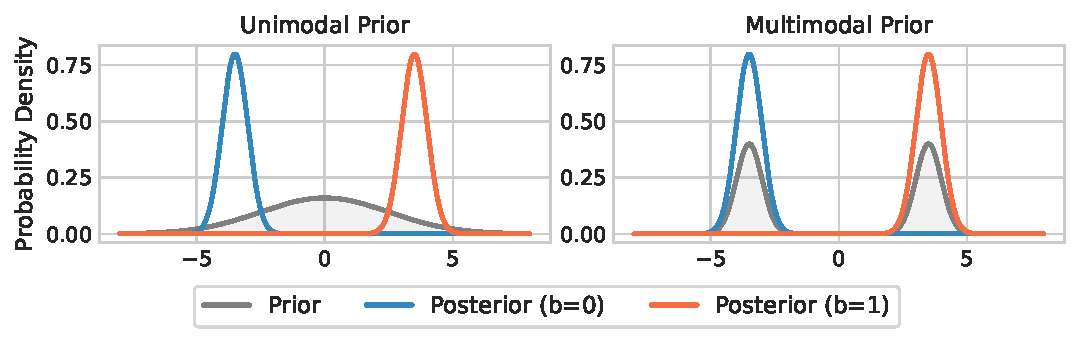
\includegraphics[width=0.85\columnwidth,keepaspectratio]{figures/unimodal_vs_multimodal_prior.pdf}
    \caption{Visualization of posteriors for transmitting a bit $b$ under a unimodal Gaussian prior vs. multimodal GMM prior.}
    \label{fig:unimodal_vs_multimodal_prior}
\end{figure}

Figure~\ref{fig:unimodal_vs_multimodal_prior} visualizes posterior distributions for transmitting bits 0 or 1, along with a unimodal Gaussian prior (left) and a multimodal GMM prior (right). Transmission is significantly more efficient with a GMM prior, highlighting why such a prior is critical for constructing our family of asymptotically optimal variational codes. We provide more detailed analysis of each case below.

\paragraph{Unimodal (Gaussian) Prior} First, consider the case where the prior is a single zero-mean unit Gaussian, $\alpha(w) = \mathcal{N}(w \mid 0, 1)$. 
The KL divergence (in nats) can be computed analytically:
\begin{equation}
\text{KL}\left[ \beta(w;\mu,\sigma^2) \parallel \alpha(w) \right] = \frac{1}{2} \left[ \sigma^2 + \mu^2 - 1 - \log(\sigma^2) \right]
\end{equation}
To make the transmission reliable, the mean $\mu$ must be sufficiently far from $0$ and the variance $\sigma^2$ must be sufficiently small. However, increasing $\mu \gg 0$ or decreasing $\sigma^2 \ll 1$ both increase the KL divergence. Therefore, we must tradeoff the KL divergence with the probability of correct decoding, with the Pareto frontier visualized in Figure~\ref{fig:unimodal_vs_multimodal_frontier}. Reaching a probability of correct decoding close to 1 requires a KL of $\gg 1$ bits.


\begin{figure}[h!]
    \centering
    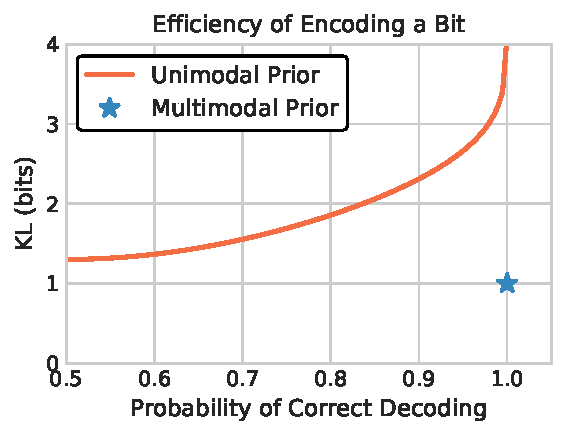
\includegraphics[width=0.5\columnwidth,keepaspectratio]{figures/unimodal_vs_multimodal_frontier.pdf}
    \caption{With a unimodal prior, we must tradeoff the KL divergence of the posterior against the expectation that the sign of the sampled parameter matches the sign of a given bit. With a multimodal prior, we can optimally encode the bit.}
    \label{fig:unimodal_vs_multimodal_frontier}
\end{figure}

\paragraph{Multimodal (GMM) Prior}
Now, let the adaptive prior be a two-component Gaussian Mixture Model (GMM) with equal weights, means $-1$ and $1$, and variance $\hat{\sigma}^2 \approx 0$.
\begin{equation*}
\alpha(w) = \frac{1}{2} \mathcal{N}(w; -1, \hat{\sigma}^2) + \frac{1}{2} \mathcal{N}(w; 1, \hat{\sigma}^2)
\end{equation*}

To send a bit $b=1$ or $b=0$, Alice can choose a posterior with mean $1$ or $-1$, respectively, and variance $\hat{\sigma}^2$.
Consider the $b=1$ case. Since $\hat{\sigma}^2 \approx 0$, the probability of correct decoding is $\approx 1$.
Additionally, the probability of any value sampled from the posterior $\beta(w;1,\hat{\sigma}^2)$ according to the prior mixture component with mean $-1$ is negligible, so the KL divergence then simplifies to be the KL divergence between the posterior and the prior component at $1$:
\begin{align*}
\text{KL}[\beta(w;1,\hat{\sigma}^2) \parallel \alpha(w)] &= \mathbb{E}_{w \sim \beta(w;1,\hat{\sigma}^2)} \left[ \log_2 \frac{\beta(w;1,\hat{\sigma}^2)}{\alpha(w)} \right] \\
&\approx \mathbb{E}_{w \sim \beta(w;1,\hat{\sigma}^2)} \left[ \log_2 \frac{\mathcal{N}(w; 1, \hat{\sigma}^2)}{\frac{1}{2} \cdot \mathcal{N}(w; 1, \hat{\sigma}^2)} \right] \\
&= \mathbb{E}_{w \sim \beta(w;1,\hat{\sigma}^2)} [\log_2 2] = 1 \text{ bit}.
\end{align*}

Thus, we can transmit the bit with an optimal KL cost of 1 bit, with near certain probability of correct decoding, as shown in Figure~\ref{fig:unimodal_vs_multimodal_frontier}. 

\subsubsection{Optimal Mixture Priors}\label{sec:optimal-mixture-priors}

In this section we discuss how adaptive GMM priors enable efficient encoding of quantized weights, as previously discussed in \citet{ullrich2017soft} and \citet{nowlan1992simplifying}.
Specifically, we will derive the optimal GMM prior parameters for the following case:
\begin{itemize}
    \item We have a group of $N$ weights with a shared, adaptive GMM prior with $K$ mixture components (\ref{sec:gaussian-parameterization}).
    \item We want to optimize the KL divergence between this prior and a posterior over these weights.
    \item The posterior for each weight approximates a delta function at a particular value.
    \item These posterior delta functions are all clustered at a small set of $M \leq K$ unique values. Let $\{m_1, m_2, \cdots, m_M\}$ denote these unique values, and let $c_i$ be the count of weights that have the value $m_i$, such that $\sum_{i=1}^M c_i = N$.
\end{itemize}
The optimal GMM prior (that minimizes KL divergence) is a mixture of $M$ components, where each component is a Dirac delta function centered at one of the unique value $m_i$. The remaining $K-M$ components should have a mixing weight of zero. Specifically, the optimal parameters, $\{(\mu_k, \nu_k, w_k)\}_{k=1}^K$, for this prior are:
\begin{itemize}
    \item \emph{Means}: The mean of each active component is set to one of the unique weight values. For $i = 1, \dots, M$, the optimal mean is $\mu_i = m_i$.
    \item \emph{Variances}: As the components converge to Dirac delta functions, their variances must approach zero. Thus, the optimal softplus parameter is $\nu_i \to -\infty$, which implies $\sigma_i^2 \to 0$.
    \item \emph{Mixing coefficients}: The mixing coefficient for each active component should be equal to the empirical frequency of the corresponding unique value in the data. For $i = 1, \dots, M$, we select $w_i$ such that the optimal mixing coefficient is $\pi_i = \frac{c_j}{N}$. The mixing coefficients for the remaining $K-M$ components are zero.
\end{itemize}

 By using a GMM with delta function components, the prior perfectly matches the empirical distribution of the weights, leading to the minimum KL divergence.
In this idealized setting, the total KL divergence is equivalent to the Shannon entropy of the empirical distribution of the weights, scaled by the total number of weights $N$. Let $p_i = c_i / N$ be the empirical frequency of the unique weight value $m_i$. The KL divergence for a single weight whose posterior is a delta function at $m_i$ simplifies to the negative log-likelihood under the prior, $-\log_2 \alpha(m_i)$. Since the optimal prior sets $\alpha(m_i) = p_i$, the cost for this single weight is $-\log_2 p_i$. Summing this cost over all $N$ weights in the group, we get the total KL divergence:
\begin{equation*}
\sum_{i=1}^{M} c_i (-\log_2 p_i) = \sum_{i=1}^{M} N p_i (-\log_2 p_i) = N \left( -\sum_{i=1}^{M} p_i \log_2 p_i \right) = N \cdot H(p)
\end{equation*}
where $H(p)$ is the Shannon entropy of the empirical distribution $p = (p_1, \cdots, p_M)$. This is the theoretical minimum number of bits required to encode the specific weight values given their empirical frequencies.

This highlights a close connection between the dynamic quantization method of \citet{han2016deep}, as employed by \citet{lotfi2022pac,lotfi2024non}, and this special case of optimizing a variational objective with an adaptive GMM prior.

\subsection{Proof of Theorem~\ref{thm:gmm-code-is-optimal}}
\label{sec:transformer-var-code-details}

\begin{thm*}[Theorem~\ref{thm:gmm-code-is-optimal} restated] There exists an asymptotically optimal family of adaptive variational codes for Transformer encoders where the adaptive prior and posterior distributions are both specified by products of independent GMMs.
\end{thm*}

\begin{proof}
We construct a family of adaptive variational codes $\{ M_R \mid R \in \gR \}$ and show it is asymptotically optimal with respect to a universal prefix Turing machine $T \in \gT$.

\paragraph{Construction of the code family}
For each resource bound $R \in \gR$, the code $M_R$ is defined as follows.
The hypothesis space $\gH_{M_R}$ consists of the weights for a Transformer encoder architecture that uses layerwise weight sharing, as specified by the construction of $\zmap(T,R,z)$ in Section~\ref{sec:zmap-details}. For a given $h \in \gH_{M_R}$, let $h_i \in h$ denote the specific Transformer weight value for some index $i$, assuming some arbitrary enumeration of the weights.
The mapping function $m_{M_R}$ is also as defined in that section, prepending $R_s$ prompt tokens to the input before the Transformer forward pass. 

The prior and posterior hypotheses spaces, $\Psi_{M_R}$ and $\Phi_{M_R}$, are both parameterized by sets of independent Gaussian mixture models (GMMs), as described in Section~\ref{sec:gaussian-parameterization}. For posterior parameters $\phi \in \Phi_{M_R}$, let $\phi_i$ denote the parameters of a GMM with index $i$. Similarly, for adaptive prior parameters $\psi \in \Psi_{M_R}$, let $\psi_{\texttt{group}(i)}$ denote the parameters of a GMM with index $\texttt{group}(i)$, where $\texttt{group}: \N \rightarrow \N$ is a function defining a grouping of Transformer weights that share the same prior GMM. 

The posterior distribution is defined as:
\begin{equation}
    \beta_{M_R}(h; \phi) = \prod_i \text{GMM}(h_i; \phi_i).
\end{equation}
The adaptive prior distribution is similarly defined as:
\begin{equation}
    \alpha_{M_R}(h; \psi) = \prod_i \text{GMM}(h_i; \psi_{\texttt{group}(i)}).
\end{equation}
Recall that the number of weights in the Transformer constructed by $\zmap$ is finite, except for the number of prompt token embeddings, where the number of rows (i.e. number of prompt tokens) grows with the space resource bound $R_s$, and therefore our asymptotic analysis largely focuses on these weights (see \ref{sec:prompt-embeddings}).

For the prompt token embeddings, a separate GMM prior is shared across each feature column.
For all weights other than the prompt token embeddings, this grouping does not formally affect our results, e.g. we can simply share a single GMM prior across each matrix or bias vector in the Transformer. 

We require that the prior and posterior GMMs corresponding to the weights of the prompt embedding table have at least $2$ components. We will show that the other GMMs only formally require a single component for the desired asymptotic bounds to hold, although a prior with more components can lead to a more efficient code in practice, as discussed below.

Finally, we construct the encoding of the prior parameters, $L_{M_R}^\Psi$, as follows. Our constructed grouping of weights sharing the same prior ensures that the total number of prior parameters in $\Psi_{M_R}$ is a small constant that does not depend on the resource bound $R$. This is because the number of parameters generated by $\zmap$ is constant with respect to $R$, other than the number of rows in the prompt token embedding table, and a single prior for each column is shared across every row of the prompt embedding table. Assuming the prior parameters can be encoded with some finite precision, we select some uniform encoding for the prior parameters, $L_{M_R}^\Psi$, which assigns non-zero probability to any specific set of prior parameters we construct below, such that they can be transmitted in $c_\Psi$ bits, which does not depend on $R$.

\paragraph{Proof of asymptotic optimality}
To prove that the family $\{M_R : R \in \gR \}$ is asymptotically optimal, we must show that for any resource bound $R \in \gR$ and any dataset $X,Y$:
\begin{equation}
L^{\bigast,\text{adaptive-var}}_{M_R}(Y \mid X) \leqc C^{\text{two-part}}_{T,R}(Y \mid X).
\end{equation}
Recall that the minimum codelength is achieved by minimizing over all possible prior and posterior parameters,
\begin{equation*}
    L^{\bigast,\text{adaptive-var}}_{M_R}(Y \mid X) = \min_{\psi \in \Psi_{M_R},\phi \in \Phi_{M_R}} L^{\text{adaptive-var}}_{M_R}(Y \mid X;\psi,\phi),
\end{equation*} 
where,
\begin{align*}
    L_{M_R}^{\text{adaptive-var}}(Y \mid X; \psi,\phi) &= L^\psi_{M_R}(\psi) + \text{KL}\left[ \beta_{M_R}(\cdot;\phi) \parallel \alpha_{M_R}(\cdot;\psi) \right] - \log_2~ p_{M_R}(Y \mid X; \phi) \\
    &= c_\Psi + \text{KL}\left[ \beta_{M_R}(\cdot;\phi) \parallel \alpha_{M_R}(\cdot;\psi) \right] - \log_2~ p_{M_R}(Y \mid X; \phi).
\end{align*}

We will show that for any resource bound $R \in \gR$ and program $z \in \gZ_{T,R}$, we can construct a specific set of prior parameters $\psi^{R}$ -- not dependent on program $z$ -- and posterior parameters $\phi^{R,z}$ such that the resulting variational codelength satisfies the following bound with respect to the function $f_T^z$ computed by prefix Turing machine $T$ with program $z$. 
That is, we will show that there exist $\psi^{R} \in \Psi_{M_R}$ and $\phi^{R,z} \in \Phi_{M_R}$ such that:
\begin{align}
L_{M_R}^{\text{adaptive-var}}(Y \mid X, \psi^R, \phi^{R,z}) \leq c_\Psi + |z| + c_T - \log_2 p(Y \mid X; f_T^z),
\end{align}
where $c_T$ and $c_\Psi$ are constants that do not depend on $X$, $Y$, $z$, or $R$.
We address the data likelihood and KL divergence terms individually next. Then we will show that this condition implies asymptotic optimality. 

Let $h^{R,z} = \zmap(T,R,z)$ be the set of weights generated by the ALTA compiler to emulate the Turing machine $T$ with program $z$.

\paragraph{Data likelihood}

For a given program $z \in \gZ_{T,R}$, we construct posterior parameters such that any weights sampled from the posterior distribution compute $f_T^z$, i.e. any sampled weights compute the same function as the weights $h^{R,z}$.

To accomplish this, we partition the Transformer weights into two disjoint subsets, which we will denote with respect a set of indexes $\gI \in \N$. For the first subset, consisting of weights with indexes $\in \gI$, we can set the parameters of the corresponding posterior GMM $\phi^{R,z}_i$ to approximate a Dirac delta function at the desired weight value, $h^{R,z}_i$. This is possible because a GMM component's variance can approach zero (see~\ref{sec:gaussian-parameterization}). The second subset, consisting of weights with indexes $\notin \gI$, consists of only those weights in the first column of the prompt token embedding table (see~\ref{sec:prompt-embeddings}) corresponding to weights encoding the values of bits on the program tape after $z$, i.e. rows $|z| + 1$ to $R_s$. By construction, these parameters are never ``read'' by the attention head scanning the program tape, so their value does not affect the function being computed by the Transformer. We therefore allow these weights to take on a ``random'' value by setting the corresponding posterior parameters to approximate the Rademacher distribution. This construction allows these bits to be transmitted ``for free'', as we will show in the next section. Formally, the posterior distribution specified by the posterior parameters $\phi^{R,z}$ is therefore:
\begin{equation}
    \text{GMM}(w;\phi^{R,z}_i) = 
    \begin{cases} 
    \delta(w - h_i^{R,z}) &, i \in \gI \\
    \frac{1}{2}\delta(w + 1) + \frac{1}{2}\delta(w - 1) &, i \notin \gI \\
    \end{cases}.
\end{equation}
Therefore, given the posterior parameters $\phi^{R,z}$, the negative log likelihood of the data is equivalent to that under a two-part code with weights $h^{R,z}$:
\begin{align}
-\log_2 p_{M_R}(Y \mid X; \phi^{R,z}) &= 
\mathbb{E}_{h \sim \beta_{M_R}(\cdot;\phi^{R,z})} \left[ -\log_2 p(Y|X; m_{M_R}(h)) \right] \\
&= -\log_2 p(Y|X; m_{M_R}(h^{R,z})) \\
&= -\log_2 p(Y|X; f_T^z).
\end{align}

\paragraph{KL divergence}
We now show that we can select prior parameters $\psi^{R} \in \Psi_{M_R}$ such that the KL divergence term is bounded by $|z| + c_T$, where $c_T$ is a constant depending only on $T$ but not on $z$ or $R$. Because the prior and posterior are parameterized by \emph{independent} GMMs, the overall KL computation factors across the individual weights of the Transformer:
\begin{equation}
    \text{KL}\left[ 
    \beta(\cdot;\phi^{R,z}) \parallel 
    \alpha(\cdot;\psi^{R}) \right] = \sum_i \text{KL}\left[  \beta(\cdot;\phi^{R,z}_i)
    \parallel
    \alpha(\cdot;\psi^{R}_{\texttt{group}(i)})
    \right]
\end{equation}
We consider the weights in the prompt embedding table first, and then discuss the remaining weights.
Recall that a GMM prior is shared for each column in this table. The weights in the first column encodes the contents of the program tape. We set the prior for this first column of the program embedding table to approximate the Rademacher distribution, such that the prior and posterior distribution are the same for the weights corresponding to the $R_s - |z|$ rows in the table after row $|z|$. The KL divergence between two equal distributions is $0$. For the weights in the first $|z|$ rows, the posterior is either a delta function at $1$ or $-1$. In either case, the KL divergence is $1$ bit (see \ref{sec:unimodal-vs-multimodal-priors}, which also highlights the importance of a \emph{multimodal} prior in our construction). For the remaining columns of the prompt embedding table, each row has the same value, and the posterior for all rows within a column approximates a delta function at this value. Therefore, we can set the prior to be equal to the posterior, and the KL divergence is $0$ for these weights. Therefore, the overall KL divergence for the prompt embedding table is $|z|$.

For the finite set of weights outside of the prompt embedding table, the posterior distribution for each weight approximates a delta function. The weights generated by $\zmap$ contain a relatively small set of unique values determined by $T$. We can choose any prior that assigns non-zero probability to these specific weight values. Summing over all fixed weights gives a total constant cost $c_T$ that depends on $T$ but not on $z$ or $R$. 
A single mixture component is formally sufficient, since it can have sufficiently large variance to assign non-zero probability to each unique value in the corresponding weight matrix. However, since the weight values generated by $\zmap$ have values drawn from a finite set determined by $T$, with a sufficient number of components, we can construct the shared GMM priors to be mixtures of delta functions centered at these values, as described in \ref{sec:optimal-mixture-priors}, and therefore $c_T$ can be relatively small.

Combining these parts, the total KL divergence is $|z| + c_T$.

\paragraph{Conclusion}
We have shown that for any program $z \in \gZ_{T,R}$ and resource bound $R \in \gR$, there exists a choice of prior and posterior parameters $(\psi^R, \phi^{R,z})$ such that:
\begin{equation}
L_{M_R}^{\text{adaptive-var}}(Y \mid X, \psi^R, \phi^{R,z}) \leq - \log_2 p(Y \mid X; f_T^z) + |z| + c_T + c_\Psi.
\end{equation}

The minimum codelength for the family $M_R$ is found by minimizing over all $(\psi, \phi)$, so it must be less than or equal to the codelength for this specific choice, minimized over all programs $z$:
\begin{align*}
L^{\bigast,\text{adaptive-var}}_{M_R}(Y \mid X) &= \min_{\psi \in \Psi_{M_R},\phi \in \Phi_{M_R}}~ L^{\text{adaptive-var}}_{M_R}(Y \mid X;\psi,\phi) \\
&\leq \min_{z \in \gZ_{T,R}} L^{\text{adaptive-var}}_{M_R}(Y \mid X;\psi^R,\phi^{R,z}) \\
&\leq \min_{z \in \gZ_{T,R}} \left( c_\Psi + |z| + c_T - \log_2 p(Y \mid X; f_T^z) \right) \\
&\leqc \min_{z \in \gZ_{T,R}} \left( |z| - \log_2 p(Y \mid X; f_T^z) \right)
\end{align*}

This last expression is equal to the definition of $C^{\text{two-part}}_{T,R}(Y \mid X)$:
\begin{align*}
C^{\text{two-part}}_{T,R}(Y \mid X) 
&= \min_{f \in \gF} \left( K_{T,R}(f) - \log_2 p(Y \mid X; f) \right) \\ 
&= \min_{z \in \gZ_{T,R}} \left( |z| - \log_2 p(Y \mid X; f_T^z) \right).
\end{align*}

Therefore our construction satisfies the condition for an asymptotically optimal family of codes.
\end{proof}


\subsection{Analysis of Alternative Two-Part Codes}
\label{sec:quasi-optimal}

Here we provide additional details and discussion related to the bounds in Table~\ref{tab:asymptotic-bounds} introduced in Section~\ref{sec:asymptotic-bounds}. The first row of the table shows a description length bound of $|z| + \log R_s$, leading to an overall codelength bound:
\begin{equation}
    L^{\bigast}_{M_R}(Y \mid X) \leqc C^{\text{two-part}}_{T,R}(Y \mid X) + \log_2 R_s.
\end{equation}

First let us detail the construction of this family of two-part codes in contrast to the construction of the variational code detailed in \ref{sec:transformer-var-code-details}.
One of the key challenges addressed by the adaptive variational code is that we wanted to transmit the $R_s$ prefix token embeddings representing the program tape contents in $|z|$ bits in order to satisfy the conditions of asymptotic optimality. In order for the ``unused'' capacity to be transmitted ``for free'', our proposal required a multimodal GMM posterior that could be set equal to the prior for the $R_s - |z|$ ``unused'' weights. However, implementing and optimizing a multimodal posterior can be challenging. Instead, Alice can adaptively determine the optimal prefix length by selecting $|z| \in \{1, \cdots, R_s \}$, e.g. by sweeping over prefix length as a hyperparameter, using structured dropout, or using some other approach. Alice can then communicate $|z|$ to Bob in $\log_2 R_s$ bits, assuming a naive uniform prior over the integers $\{ 1, \cdots, R_s \}$ for encoding $|z|$. Then, Alice can simply communicate $z$ in $|z|$ bits assuming a Rademacher prior over the $|z|$ weights, as in our previous construction in \ref{sec:transformer-var-code-details}. As in our previous construction, this can be generalized by using an adaptive GMM prior. Alternatively, such a code could potentially be constructed using the quantization method of \citet{han2016deep}, which has also been employed by \citet{lotfi2022pac,lotfi2024non}. Alternatively, we could restrict the prefix embeddings to some fixed vocabulary, akin to discrete prompt optimization. Most directly, in the special case where the vocabulary size is $2$, we reach the same bound. 


Next we discuss the bounds in Table~\ref{tab:asymptotic-bounds} resulting from ablating aspects of this recipe. First, if we do not use any form of quantization, and instead use a fixed prior, such as the unimodal Gaussian prior implicit in methods such as weight decay, or a uniform prior implicit in standard MLE objectives, then each weight encoding a bit of $z$ requires more than a single bit to encode. Therefore, the program length term in the bound changes from $|z|$ to $\gO(|z|)$, where the multiplicative factor is $>1$. Second, if we do not adaptively select the prefix length, then we must encode the entire prefix embedding table, which contains $R_s$ rows, regardless of the length of the program it encodes. Therefore, the bound degrades further to $\gO(R_s)$, where $R_s \geq |z|$ as by definition $R_s$ determines the maximum program length that can be represented. Finally, if we do not use layerwise weight sharing, then our bound simply becomes a function of the number of parameters in the Transformer. As $R_t$ specifies the number of layers, we must encode $\gO(R_t)$ weights, in addition to the $\gO(R_s)$ weights in the prefix embedding table. Note that the bounds we have derived assume we are using the Transformer family and specification of $\zmap$ discussed in Section~\ref{sec:two-part-codes-for-transformers}. Alternative constructions could potentially lead to different bounds.

Overall, a weaker bound on the model description length leads to a weaker bound on the minimum of the overall codelength. Therefore, optimizing such an objective may lead to sub-optimal compression, and---from an MDL perspective---sub-optimal model selection. Regardless, the $|z| + \log R_s$ bound is close to the theoretically optimal bound of $|z|$. While pre-trained Transformer decoders are a different setting than the one we have studied here, if our results could be extended to that setting it would provide a strong asymptotic bound for the compression achievable via prompt optimization methods, complementing the positive empirical results from~\citet{akinwande2024understanding}.

\subsection{Scaling Transformer Dimensionality}
\label{sec:mlp-scaling}

Here we provide additional details on the alternative Transformer family discussed in Section~\ref{sec:alternative-families}. In contrast to the Transformer family detailed in \ref{sec:zmap-details}, the program tape contents are implicitly encoded in the MLP parameters. In this construction, we still require prepending $R_s$ ``padding'' tokens to the input in order to scale the context window so that the Transformer can represent Turing machine tapes of size $R_s$. However, the program $z$ is encoded in the MLP layer, and we do not require a prefix embedding table. An ALTA program for populating the program tape contents based on a program encoded in the MLP weights is shown in Figure~\ref{fig:populate_program}. The overall construction first iteratively populates the program tape contents at sequential Transformer positions, and then the Turing machine emulation continues as in our previous construction. Therefore, this construction requires $R_t + R_s + 2$ layers.

\begin{figure}[h!]
\centering
\begin{minted}[
  frame=single,
  framesep=2mm, 
  fontsize=\fontsize{8}{9}\selectfont\ttfamily,
  ]{python}
from alta import program_builder as pb

def build_program_spec(program_input: list[int]) -> pb.ProgramSpec:
  """Returns ALTA program spec for populating program tape."""

  variables = {
      "done": pb.var(2),
      "is_start": pb.input_var(2, init_fn=lambda x: x == START),
      "head": pb.input_var(2, init_fn=lambda x: x == START),
      "symbol": pb.input_var(2),
      "program_index": pb.var(len(program_input)),
  }
  attention_heads = {
      "head_left": pb.v_relative("head", -1),
  }

  def ffn_fn(x):
    if x["program_index"] == len(program_input):
      x["done"] = 1
      return

    if x["head"]:
      x["symbol"] = int(program_input[x["program_index"]])
      x["head"] = 0

    if not x["is_start"] and x["head_left"]:
      x["head"] = 1

    x["program_index"] = x["program_index"] + 1

  return pb.program_spec(
      ffn_fn=ffn_fn, variables=variables, heads=attention_heads,
      output_name="symbol", input_range=2, position_range=None,
  )
\end{minted}
\caption{ALTA program specification for populating a program tape given a program encoded in the MLP layer.}
\label{fig:populate_program}
\end{figure}


The MLP matrices generated by the ALTA program in Figure~\ref{fig:populate_program} require $\gO(|z|^2)$ parameters, and have rank $\gO(|z|)$, where $|z|$ is the program length. While the existence of a mapping analogous to $\zmap$ for this Transformer family indicates that asymptotically optimal description length objectives exist, implementing such a prior introduces complex dependencies across the parameters of the MLP. Given the rank requirements on the MLP matrices under this construction, rank factorization would not be an effective means of compression, but it would be interesting for future work to consider alternative constructions or practical methods for matrix compression that could yield asymptotic bounds approaching the theoretical ideal.